\documentclass[aspectratio=169]{beamer}
\usepackage[no-math,deluxe]{luatexja-preset}
\renewcommand{\kanjifamilydefault}{\gtdefault}
\usepackage{minted}
\usepackage{xcolor}
\usepackage{hyperref}
\usepackage{amsmath}
\setbeamertemplate{navigation symbols}{}

\title{テスト駆動開発 ハンズオン \#1}
\subtitle{Test-Driven Development Hands-On \#1}
\author{ASUKA Y}
\date{Aug 21 2022}

\begin{document}

\begin{frame}
  \titlepage
\end{frame}

\section*{INDEX}
\begin{frame}
  \frametitle{テスト駆動揮発ハンズオン \#1}
  \tableofcontents
\end{frame}

\section{テスト駆動開発とは何か}
\subsection{テスト駆動開発とは何か}
\begin{frame}\frametitle{テスト開発とは何か}
  \begin{quote}
    テスト駆動開発(TDD)はテスト技法ではない...
    TDDは分析器用であり、設計技法であり、
    実際には開発のすべてのアクティビティを構造化する技法なのだ。
  \end{quote}
  \begin{flushright}
    ---Kent Beck
  \end{flushright}

  テスト技法ではなく、開発技法である。

  {
    \large \color{blue}
    $\rightarrow$
    テストを書くことが目的ではない。
  }
\end{frame}

\subsection{テスト駆動開発が目指すもの}
\begin{frame}\frametitle{テスト駆動開発が目指すもの}
  \begin{quote}
    「動作するきれいなコード」。
    Ron Jeffiresのこの簡潔な言葉が、
    テスト駆動開発(TDD)のゴールだ。
    動作するきれいなコードはあらゆる意味で価値がある。
  \end{quote}
  \begin{flushright}
    ---Kent Beck
  \end{flushright}

  TDDは動作する「きれいなコード」に辿り着くために、
  {\color{blue} 自動化されたテストによって開発を推し進める技法}である。

  \begin{center}
    \color{red} \large テストを手段として用いるのであって、テストが目的なのではない。
  \end{center}
\end{frame}

\begin{frame}[fragile]\frametitle{動作するきれいなコード}
  \begin{itemize}
    \item {\color{blue} 開発が予測可能になる。}
      何が完成していて、何が完成していないかがわかる。
    \item {\color{blue} コードが伝えようとしていることを余すところなく受け取れる。}
      最初に思いついたコードを書き殴っただけで終わりなら、
      最高してより良いコードを書くチャンスは永遠に来ない。

    \large \color{blue}
    \item あなたが作るソフトウェアのユーザを快適にする。
    \item チームメイトはあなたを信頼し、あなたもまたチームメイトを信頼する。
    \item 書いていて気持ちがいい。
  \end{itemize}
\end{frame}

\subsection{テスト駆動開発の進め方}
\begin{frame}\frametitle{テスト駆動開発の進め方}
  \begin{enumerate}
    \item まずはテストを1つ書く
    \item すべてのテストを走らせ、新しいテストの失敗を確認する
    \item 小さな変更を行う
    \item すべてのテストを走らせ、すべて成功することを確認する
    \item リファクタリングを行って重複を排除する
  \end{enumerate}

  \begin{center}
    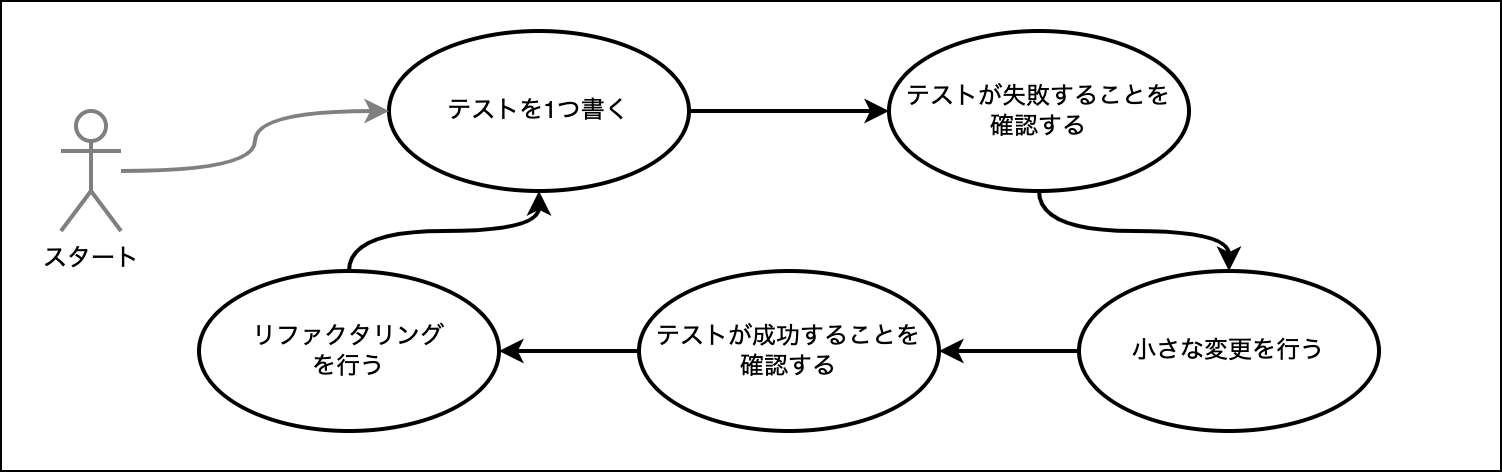
\includegraphics[height=4cm]{asset/tdd_cycle.png}
  \end{center}
\end{frame}

\begin{frame}[fragile]\frametitle{1. まずはテストを1つ書く}
  これから何を開発しないといけないのか、をはじめに考える。

  \begin{quote}
    \color{blue}
    2つの整数の和を知りたい。
  \end{quote}
  $\rightarrow$ 2つの引数を取って、和を返す関数を作れば良いんだな。

  \scriptsize
  \begin{minted}{go}
    /*-- lib.go --*/
    func Add(a, b int) int {
        return 0
    }

    /*-- lib_test.go --*/
    func TestAdd(t *testing.T) {
        result := Add(3, 4)
        if result != 7 {
            t.Fatalf("want=%d, got=%d", 7, result)
        }
    }
  \end{minted}

  {\color{gray}(\url{https://github.com/a-skua/tdd-handson/commit/89356e89595b1b403f563fc749eaeb59b15ec5b1})}
\end{frame}

\begin{frame}[fragile]\frametitle{2. 全てのテストを走らせ、新しいテストの失敗を確認する}
  {
    \color{gray}
    \scriptsize
    \begin{minted}{text}
      example % go test -cover .
      --- FAIL: TestAdd (0.00s)
          lib_test.go:10: want=7, got=0
      FAIL
      coverage: 100.0% of statements
      FAIL	github.com/a-skua/tdd-handson/example	0.199s
      FAIL
    \end{minted}
  }

  テストの失敗を確認することには意味がある。
  \begin{itemize}
    \item {\color{blue} テストが有効であることの確認。}
    \item {\color{blue} 課題(TODO)であることの明記。}
  \end{itemize}
\end{frame}

\begin{frame}[fragile]\frametitle{テストが有効であることの確認}
  成功パターンを書いていると気がつけない場合がある。
  {
    \scriptsize
    \begin{minted}{go}
      /*-- lib.go --*/
      func Add(a, b int) int {
          // 簡単な内容なので、失敗を確認せずに書き上げた
          return a + b
      }

      /*-- lib_test.go --*/
      func TextAdd(t *testing.T) {
          result := Add(3, 4)
          want := 7
          if result != want {
              t.Errorf("result=%d, want=%d", result, want)
          }
      }
    \end{minted}
  }
  {
    \scriptsize
    \color{gray}
    \begin{minted}{text}
      example % go test -cover ./...
      ok  	github.com/a-skua/tdd-handson/example	0.298s	coverage: 83.3% of statements
    \end{minted}
  }
  上記のように{\color{blue} Test}を{\color{red} Text}とTypoしてしまっていても、
  これは失敗しない。
  そして、初めから失敗を想定していないので、当然テストはパスする。
\end{frame}

\begin{frame}\frametitle{課題(TODO)であることの明記}
  失敗するテストは道標となる。
  \begin{itemize}
    \item
      翌日やることとして失敗するテストを書いておくと、
      今日は何をするのか思い出す手間が省ける。

    \item
      作業中に差し込みで別の作業が入った場合でも
      再開する時のコンテキストスイッチを素早く行える。
  \end{itemize}
\end{frame}

\begin{frame}[fragile]\frametitle{3. 小さな変更を行う}
  {
    \scriptsize
    \begin{minted}{go}
      /*-- lib.go --*/
      func Add(a, b int) int {
          return a + b
      }
    \end{minted}

    {\color{gray} (\url{https://github.com/a-skua/tdd-handson/commit/1b5250883b7d0e0b69381fb743312e680bb718c4})}
  }

  小さな変更にとどめることは非常に重要。

  一度の変更が小さければ小さいほど、
  どこで間違えたのか判断しやすくなる。
\end{frame}

\begin{frame}[fragile]\frametitle{4. 全てのテストを走らせ、全て成功することを確認する}
  \scriptsize
  \color{gray}
  \begin{minted}{text}
    example % go test -cover .
    ok  	github.com/a-skua/tdd-handson/example	0.226s	coverage: 100.0% of statements
  \end{minted}
\end{frame}

\begin{frame}[fragile]\frametitle{5. リファクタリングを行なって重複を排除する}
  {
    \scriptsize
    \begin{minted}{go}
      /*-- lib.go --*/
      func Add(a, b int) int {
          return a + b
      }

      /*-- lib_test.go --*/
      func TestAdd(t *testing.T) {
          result := Add(3, 4)
          want := 7
          if result != want {
              t.Fatalf("want=%d, got=%d", want, result)
          }
      }
    \end{minted}
  }
  1つ目の課題を完了。
  これで1サイクルが終了する。
\end{frame}

\begin{frame}[fragile]\frametitle{Re: 1. まずはテストを1つ書く}
  2サイクル目に入る

  \begin{quote}
    \color{blue}
    3つの整数の和も知りたい。
  \end{quote}
  $\rightarrow$ 3つの引数を取って、和を返す関数を作れば良いんだな。

  {
    \scriptsize
    \begin{minted}{go}
      /*-- lib.go --*/
      func Add3(a, b, c int) int {
          return 0
      }

      /*-- lib_test.go --*/
      func TestAdd3(t *testing.T) {
          result := Add(3, 4, 5)
          if result != 12 {
              t.Fatalf("want=%d, got=%d", 12, result)
          }
      }
    \end{minted}

    {\color{gray} (\url{https://github.com/a-skua/tdd-handson/commit/822b7d65a81c842db6ed62d9dc600b29c30e760c})}
  }

  コードを書き始める前から最適化について考えない方が良い。
\end{frame}

\begin{frame}[fragile]\frametitle{Re: 2. 全てのテストを走らせ、新しいテストの失敗を確認する}
  {
    \scriptsize
    \color{gray}
    \begin{minted}{text}
      example % go test -cover .
      --- FAIL: TestAdd3 (0.00s)
          lib_test.go:17: want=12, got=0
      FAIL
      coverage: 100.0% of statements
      FAIL	github.com/a-skua/tdd-handson/example	0.233s
      FAIL
    \end{minted}
  }

  テストが有効であることを確認する。
\end{frame}

\begin{frame}[fragile]\frametitle{Re: 3. 小さな変更を行う}
  \scriptsize
  \begin{minted}{go}
    /*-- lib.go --*/
    func Add3(a, b, c int) int {
        return a + b + c
    }
  \end{minted}

  {\color{gray} (\url{https://github.com/a-skua/tdd-handson/commit/1ad0b944d4b88829b820cec4b29b67bc553d99ff})}
\end{frame}

\begin{frame}[fragile]\frametitle{Re: 4. 全てのテストを走らせ、全て成功することを確認する}
  \scriptsize
  \color{gray}
  \begin{minted}{text}
    example % go test -cover .
    ok  	github.com/a-skua/tdd-handson/example	0.226s	coverage: 100.0% of statements
  \end{minted}
\end{frame}

\begin{frame}[fragile]\frametitle{Re: 5. リファクタリングを行なって重複を排除する}
  {
    \scriptsize
    \begin{minted}{go}
      /*-- lib.go --*/
      package example

      func Add(a, b int) int {
          return sum(a, b)
      }

      func Add3(a, b, c int) int {
          return sum(a, b, c)
      }

      func sum(ns ...int) (result int) {
          for _, n := range ns {
              result += n
          }
          return
      }
    \end{minted}

    {\color{gray} (\url{https://github.com/a-skua/tdd-handson/commit/e0794b19678b66cc6aa959ad73f4be367c4a2ae2})}
    \color{gray}
    \begin{minted}{text}
      example % go test -cover .
      ok  	github.com/a-skua/tdd-handson/example	0.213s	coverage: 100.0% of statements
    \end{minted}
  }
  これで2サイクル目も終了する。
\end{frame}

\subsection{テスト駆動開発がもたらすもの}
\begin{frame}\frametitle{テスト駆動開発がもたらすもの}
  \begin{itemize}
    \item {\color{blue} テストが常に再現可能である。}
    \item {\color{blue} 1サイクル完了した時点で常にすべてのテストが完了している。}
  \end{itemize}

  テスト駆動開発は大規模な開発において間違いなくエンジニアを導く灯火となり得る。
  \color{gray} 
  バグ指摘の修正対応を行う度に新たなバグ指摘をされる経験があるのであれば、
  間違いなくTDDを実践する価値はある。
\end{frame}

\begin{frame}\frametitle{テストが常に再現可能である}
  {\color{blue}「テスト = 再現可能な動作確認」}である。

  テストを実行すれば新しい実装だけでなく、すべての動作確認をすることができる。
  それぞれのアーミーナイフに頼った動作確認ではなく、
  {\color{blue} テストによってすべての環境で再現可能な動作確認が可能となる。}
\end{frame}

\begin{frame}\frametitle{1サイクル完了した時点で常にすべてのテストが完了している}
  ここまでのテストのcoverageが常に100\%になっていることに注目してほしい。

  TDDは実装を書き上げてからカバレッジを見ながらテストを追加するものではなく、
  \color{blue}
  実装すべきもの・課題をTODO化し、
  1つずつテストによって動作確認をしながら実装していく開発技法である。
\end{frame}

\subsection{テスト駆動開発を始めるために}
\begin{frame}\frametitle{テスト駆動開発を始めるために}
  TDDを始めるためにやるべきこと、知っておくべきことは4つある。
  \begin{itemize}
    \item {\color{blue} TDDに慣れる。}

      慣れていないと、実務で実践することに高いハードルを感じてしまうかもしれない。
      ハードルを低くすることこそ今回のハンズオンの趣旨。
    \item {\color{blue} 設計(デザインパターン)を知る。}
    \item {\color{blue} 何のためにテストを書くのか理解する。}
    \item {\color{blue} 美食家になる。}
  \end{itemize}
\end{frame}

\begin{frame}[fragile]\frametitle{TDDに慣れる}
  TDDを始める前と後ではコードの書き方が大きく変わることがある。
  {
    \scriptsize
    \begin{minted}{go}
      // 新しいユーザーIDを発行する
      // ユーザーIDは数字10桁で、数字はランダムに生成される
      func NewUserID() string {
           // 乱数の安全性についてここでは無視している
          return fmt.Sprint("%010d", rand.Int()%10000000000)
      }
    \end{minted}
  }
  $\rightarrow$
  副作用(乱数やDBなどコードの外に依存するもの)を伴うテストは難しい。
  {
    \scriptsize
    \begin{minted}{go}
      // 新しいユーザーIDを発行する
      // ユーザーIDは数字10桁で、数字はランダムに生成される
      func NewUserID(rand func() int) string {
          return fmt.Sprint("%010d", rand()%10000000000)
      }
    \end{minted}
  }
  しかし、副作用についてはTDDの手順で実装していくと解決できるかもしれない。

  \color{gray}\small
  テストしやすいコードを考えるのであれば、
  「参照透過性」についても学ぶと良い。
\end{frame}

\begin{frame}[fragile]
  $\rightarrow$ まずはテストを書く
  {
    \scriptsize
    \begin{minted}{go}
      /*-- lib.go --*/
      // 新しいユーザーIDを発行する
      // ユーザーIDは数字10桁で、数字はランダムに生成される
      func NewUserID() string {
          return ""
      }
      /*-- lib_test.go --*/
      func TestNewUserID(t *testing.T) {
          result := NewUserID()
          want := "1234567890"
          if result != want {
              t.Errorf("result=%s, want=%s", result, want)
          }
      }
    \end{minted}
  }
  {
    \color{gray}
    \scriptsize
    \begin{minted}{text}
      example % go test -cover ./...   
      --- FAIL: TestNewUserID (0.00s)
          lib_test.go:25: result=, want=1234567890
      FAIL
      coverage: 100.0% of statements
      FAIL	github.com/a-skua/tdd-handson/example	0.190s
      FAIL
    \end{minted}
  }
\end{frame}

\begin{frame}[fragile]
  $\rightarrow$ 数字10桁の文字列を返す
  {
    \scriptsize
    \begin{minted}{go}
      /*-- lib.go --*/
      // 新しいユーザーIDを発行する
      // ユーザーIDは数字10桁で、数字はランダムに生成される
      func NewUserID() string {
          return fmt.Sprintf("%010d", 1234567890)
      }
      /*-- lib_test.go --*/
      func TestNewUserID(t *testing.T) {
          result := NewUserID()
          want := "1234567890"
          if result != want {
              t.Errorf("result=%s, want=%s", result, want)
          }
      }
    \end{minted}
  }
  {
    \color{gray}
    \scriptsize
    \begin{minted}{text}
      example % go test -cover ./...
      ok  	github.com/a-skua/tdd-handson/example	0.217s	coverage: 100.0% of statements
    \end{minted}
  }
\end{frame}


\begin{frame}[fragile]
  $\rightarrow$
  多角的に検証する(三角測量)
  {
    \scriptsize
    \begin{minted}{go}
      /*-- lib.go --*/
      // 新しいユーザーIDを発行する
      // ユーザーIDは数字10桁で、数字はランダムに生成される
      func NewUserID() string {
          return fmt.Sprintf("%010d", 1234567890)
      }
      /*-- lib_test.go --*/
      func TestNewUserID(t *testing.T) {
          /* 省略 */

          // 別のパターンを試す
          result = NewUserID()
          want = "0123456789"
          if result != want {
              t.Errorf("result=%s, want=%s", result, want)
          }
      }
    \end{minted}
  }
  {
    \color{gray}
    \scriptsize
    \begin{minted}{text}
      example % go test -cover ./...
      --- FAIL: TestNewUserID (0.00s)
          lib_test.go:31: result=1234567890, want=0123456789
      FAIL
      coverage: 100.0% of statements
      FAIL	github.com/a-skua/tdd-handson/example	0.208s
      FAIL
    \end{minted}
  }
\end{frame}

\begin{frame}[fragile]
  $\rightarrow$
  乱数に置き換える
  {
    \scriptsize
    \begin{minted}{go}
      /*-- lib.go --*/
      // 新しいユーザーIDを発行する
      // ユーザーIDは数字10桁で、数字はランダムに生成される
      func NewUserID() string {
        return fmt.Sprintf("%010d", rand.Int()%10000000000)
      }
      /*-- lib_test.go --*/
      func TestNewUserID(t *testing.T) {
          /* 省略 */

          // 別のパターンを試す
          result = NewUserID()
          want = "0123456789"
          if result != want {
              t.Errorf("result=%s, want=%s", result, want)
          }
      }
    \end{minted}
  }
  {
    \color{gray}
    \scriptsize
    \begin{minted}{text}
      example % go test -cover ./...
      --- FAIL: TestNewUserID (0.00s)
          lib_test.go:25: result=1947779410, want=1234567890
          lib_test.go:31: result=3082153551, want=0123456789
      FAIL
      coverage: 100.0% of statements
      FAIL	github.com/a-skua/tdd-handson/example	0.211s
      FAIL
    \end{minted}
  }
\end{frame}

\begin{frame}[fragile]
  $\rightarrow$
  乱数に置き換える
  {
    \scriptsize
    \begin{minted}{go}
      /*-- lib.go --*/
      // 新しいユーザーIDを発行する
      // ユーザーIDは数字10桁で、数字はランダムに生成される
      func NewUserID() string {
        return fmt.Sprintf("%010d", rand.Int()%10000000000)
      }

    \end{minted}
  }
  乱数は副作用である。
  どうやって副作用を伴う関数のテストを行うべきか?
\end{frame}

\begin{frame}[fragile]
  $\rightarrow$
  ここでは副作用は外から渡すことにし、参照透過性を確保する。
  {
    \scriptsize
    \begin{minted}{go}
      /*-- lib.go --*/
      // 新しいユーザーIDを発行する
      // ユーザーIDは数字10桁で、数字はランダムに生成される
      func NewUserID(rnd func() int) string {
        return fmt.Sprintf("%010d", rand.Int()%10000000000)
      }
      /*-- lib_test.go--*/
      func TestNewUserID(t *testing.T) {
          // usage
          t.Log(NewUserID(rand.Int))

          result := NewUserID(func() int { return 1234567890 })
          want := "1234567890"
          if result != want {
              t.Errorf("result=%s, want=%s", result, want)
          }

          result = NewUserID(func() int { return 123456789 })
          want = "0123456789"
          if result != want {
              t.Errorf("result=%s, want=%s", result, want)
          }
      }
    \end{minted}
  }
\end{frame}

\begin{frame}[fragile]
  $\rightarrow$
  引数から渡される関数を利用するように書き換えることで、
  関数から副作用が排除される。
  {
    \scriptsize
    \begin{minted}{go}
      /*-- lib.go --*/
      // 新しいユーザーIDを発行する
      // ユーザーIDは数字10桁で、数字はランダムに生成される
      func NewUserID(rnd func() int) string {
        return fmt.Sprintf("%010d", rnd()%10000000000)
      }
    \end{minted}
  }
  {
    \color{gray}
    \scriptsize
    \begin{minted}{text}
      example % go test -cover ./...
      ok  	github.com/a-skua/tdd-handson/example	0.192s	coverage: 100.0% of statements
    \end{minted}
  }

  参照透過性のある関数とそのテストどの環境であっても同様の実行結果を得ることができる。
\end{frame}

\begin{frame}\frametitle{設計(デザインパターン)を知る}
  {\color{blue} 実装する上で必要なデザインパターンは押さえておく必要がある。}
  {
    \color{gray}
    デザインパターンを知らない場合、
    そもそもテスト可能なコードを書くのが困難になり得る。
  }

  GoF, Clean Architecture, DDD...など抑えておくデザインパターンは多い。

  {\color{blue} 特にDDDはTDDと合わせて抑えておきたい。}
  {
    \color{gray}
    TDDで用いるテストはプログラムの機械的な正しさよりは
    サービスドメイン上の正しさを確認できるものでありたい。
  }
\end{frame}

\begin{frame}\frametitle{サービスドメイン上の正しさ}
  TDDを実践するにあたって、ドメイン駆動設計(DDD)についても学んでおきたい。

  ソフトウェア的な階層によってコードを集約するのではなく、
  サービスの関心ごと(ドメイン)毎にコードを集約していく設計技法である。

\end{frame}

\begin{frame}\frametitle{何のためにテストを書くのか理解する}
  {\color{blue} TDDはエンジニア自身のためにある開発技法}
  であって、ユーザー(顧客)のための手法ではない。
  {\color{blue} 「テスト = 再現可能な動作確認」}
  であることを理解しておきたい。
  \begin{quote}
    \color{gray}
    リリースするには品質を担保するためにテストが書かれている必要があり、
    カバレッジをN\%以上満たしている必要がある。
  \end{quote}
  このような形骸化したルールだけがあり、
  チームの誰もがこのルールのためにテストを書いているようであれば、
  TDDを語る以前に書かれたテスト自体も意味を成していない可能性が高い。
\end{frame}

\begin{frame}\frametitle{美食家になる}
  食生活は体調の良し悪しに関わる。

  伸びきったスパゲッティを貪るような食生活をやめよう。

  腐ったものや美味しくないものに気付かずに食べているかもしれないので、
  正しい味覚を身につけよう。
\end{frame}

\section{ハンズオン}
\begin{frame}\frametitle{ハンズオン}
  {\color{gray} \url{https://github.com/a-skua/tdd-handson}}
  \begin{itemize}
    \item フィボナッチ数列
      \begin{quote}
        TDD入門
      \end{quote}
    \item 逆ポーランド記法電卓
      \begin{quote}
        少し複雑なプログラム
      \end{quote}
    \item RESTful API
      \begin{quote}
        実践的な入門
      \end{quote}
  \end{itemize}

  \color{gray}
  より複雑な実装をを試してみた人へ
  \begin{itemize}
      \color{gray}
    \item ライフゲーム
    \item JSONパーサ
  \end{itemize}
\end{frame}

\subsection{フィボナッチ数列}
\begin{frame}\frametitle{ハンズオン: フィボナッチ数列}
  {\color{gray} \url{https://github.com/a-skua/tdd-handson/tree/main/fibonacci}}

  \begin{align*}
    F_0 &= 0, \\
    F_1 &= 1, \\
    F_{n+2} &= F_n + F_{n+1} (n \ge 0)
  \end{align*}

  \begin{enumerate}
    \item まずはテストを1つ書く
    \item すべてのテストを走らせ、新しいテストの失敗を確認する
    \item 小さな変更を行う
    \item すべてのテストを走らせ、すべて成功することを確認する
    \item リファクタリングを行って重複を排除する
  \end{enumerate}
\end{frame}

\subsection{逆ポーランド記法電卓}
\begin{frame}\frametitle{ハンズオン: 逆ポーランド記法電卓}
  {\color{gray} \url{https://github.com/a-skua/tdd-handson/tree/main/calculator}}

  中置記法
  \[ (1 + 2) * (3 + 4) \]
  ポーランド記法(前置記法)
  \[ *\, +\,1\,2\, +\,3\,4 \]

  逆ポーランド記法(後置記法)
  \[ 1\,2\,+\, 3\,4\,+\, * \]

  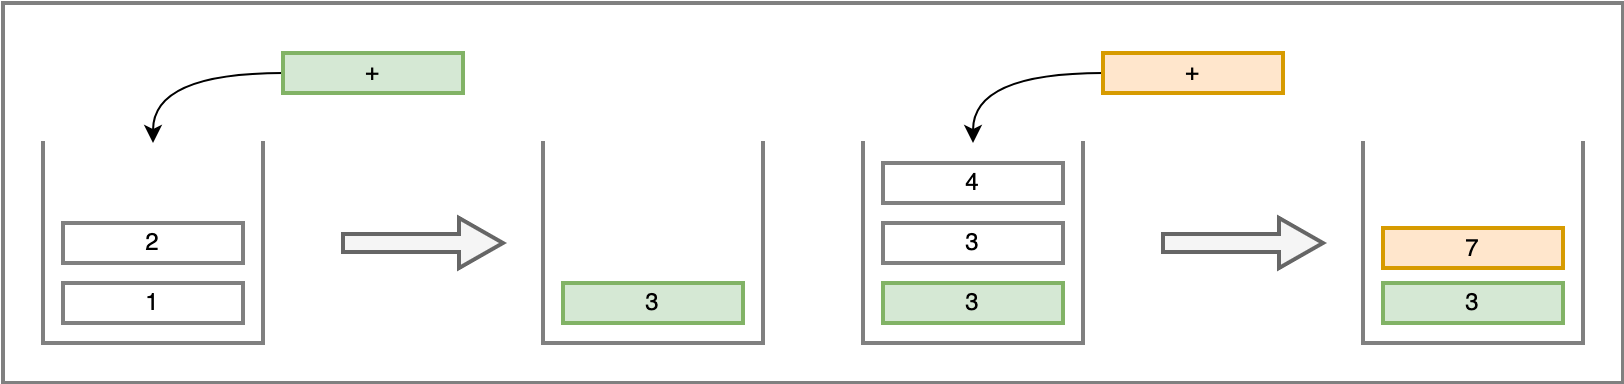
\includegraphics[height=3cm]{asset/stack.png}
\end{frame}

\subsection{RESTful API}
\begin{frame}\frametitle{ハンズオン: RESTful API}
  {\color{gray} \url{https://github.com/a-skua/go-api-example}}
  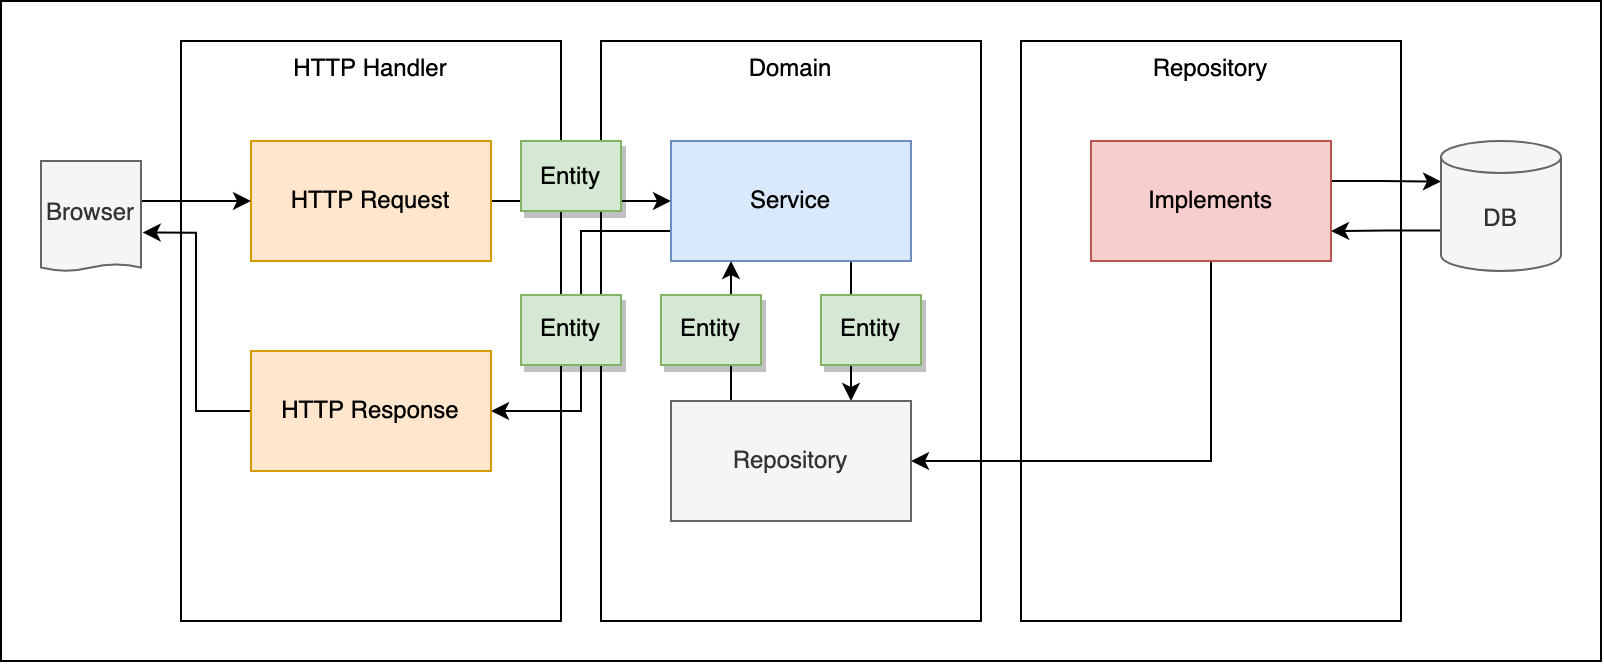
\includegraphics[height=6cm]{asset/api.png}
\end{frame}

\end{document}
